\chapter{Project Overview}

{ {{- project.customer -}} } commissioned us to perform a penetration test in the period from
{ {{- project.start_date|date('d.M.Y') -}} } to { {{- project.end_date|date('d.M.Y') -}} }.

The scope was set as follows:

\begin{itemize}
    
    \item {{ scope.name }}
    
\end{itemize}

The table \ref{tbl:host-summary} gives an overview of the systems identified during the penetration test.

\begin{table}[ht]
    \renewcommand{\arraystretch}{1.5}
    \centering
    \begin{tabularx}{\textwidth}{| X | X | X |}
        \hline
        \textbf{Host} & \textbf{OS} & \textbf{Hostnames} \\
        \hline
        
        {{ host.ip }} & {{ host.os }} & {{ host.get_hostnames() }}    \\
        \hline
        
    \end{tabularx}
    \caption{Host Overview}
    \label{tbl:host-summary}
\end{table}


As a result, vulnerabilities were found in the examined systems, which pose an increased risk.


Figure \ref{fig:bsi} shows the classification of a penetration test according to the standard model of the German Federal Office for Information Security.


\begin{figure}[h]
\centering
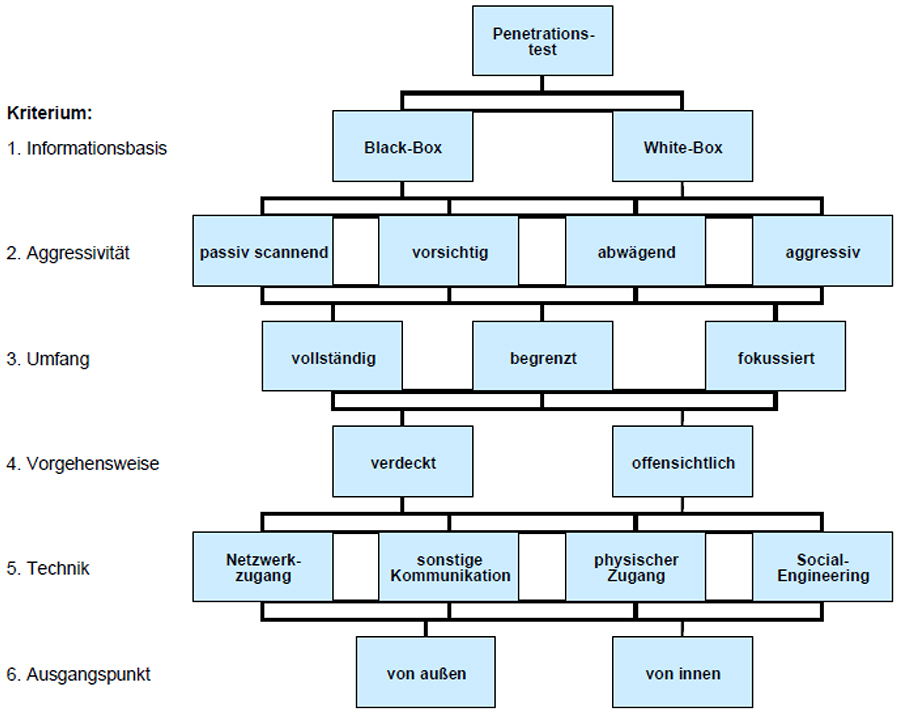
\includegraphics[scale=0.3]{bsi.jpg}
\caption{BSI Classification}
\label{fig:bsi}
\end{figure}

The criteria are explained below.

TODO